% RQ-A dissertation scaffold (Gate F1 framing, August 2026).
% The July cross-model-agreement draft is preserved unchanged in main.tex;
% this file reuses its UCL template preamble and the portable literature
% review sections. Compile from this directory with: latexmk -pdf main_v2.tex
% For two-sided printing, replace "oneside" with "twoside".
\documentclass[11pt,a4paper,oneside]{book}

\usepackage[british]{babel}
\usepackage[T1]{fontenc}
\usepackage[utf8]{inputenc}
\usepackage{amsmath,amssymb,amsthm,color,enumerate,graphicx,stackrel,natbib,setspace,ifthen,url,array,pifont}
\usepackage{lscape}
\usepackage{placeins}
\usepackage{multirow}
\usepackage{fancyhdr}
\usepackage{emptypage}
\usepackage[margin=3cm]{geometry}
\usepackage[sc]{titlesec}
\usepackage[titletoc,title]{appendix}
\linespread{1.3}

\usepackage{booktabs}
\usepackage{xcolor}
\usepackage{enumitem}
\usepackage{listings}
\usepackage{csquotes}
\usepackage[hidelinks]{hyperref}
\usepackage{doi}
\usepackage[capitalise,noabbrev]{cleveref}

% Preserve the existing citation commands while using the template's natbib
% bibliography formatting.
\let\textcite\citet
\let\Textcite\Citet
\let\parencite\citep

\definecolor{draftgrey}{gray}{0.38}
\newif\ifshowdraftnotes
\showdraftnotestrue
\newcommand{\draftnote}[1]{%
  \ifshowdraftnotes
    \par\smallskip
    \noindent{\color{draftgrey}\small\itshape Drafting note: #1\par}
    \smallskip
  \fi
}

\graphicspath{{figures/}{./}}

\setcounter{secnumdepth}{3}
\setcounter{tocdepth}{3}
\emergencystretch=3em

% Working title; settle the final wording with the supervisor.
\title{News Sentiment Beyond the Mean:\\Aggregating Same-Day Stories and Testing What Survives Costs}
\author{Peter Prendergast}
\date{September 2026}

\begin{document}
\pagestyle{plain}
\frontmatter
\hypersetup{pageanchor=false}

\begin{titlepage}
  \newcommand{\HRule}{\rule{\linewidth}{0.5mm}}
  \centering

  \textsc{\LARGE University College London}\\[1cm]
  \textsc{\Large Department of Computer Science}\\[0.4cm]
  \textsc{\large A thesis submitted in partial fulfilment of the requirements for the degree of Master of Science in Computational Finance, University College London}\\[0.4cm]

  \HRule\\[0.3cm]
  \textsc{\LARGE News Sentiment Beyond the Mean}\\[0.3cm]
  \HRule\\[1cm]

  {\large\textit{Author}}\\
  Peter \textsc{Prendergast}
  \vfill

  {\large\textit{Industry Supervisor}}\\
  {\large Dr Peter \textsc{Mitic}}\\
  {\large\textsc{Department of Computer Science}}\\
  {\large\textsc{University College London}}

  \vfill

  {\large\textit{Academic  Supervisor}}\\
  {\large Dr Brian \textsc{Healy}}\\
  {\large\textsc{Department of Computer Science}}\\
  {\large\textsc{University College London}}

  \vfill
  {\large\textit{September 2026}}

  
\includegraphics[width=0.15\textwidth]{ucl_logo}\\[0.5cm]

  \begin{minipage}{0.9\textwidth}
    \small
    This dissertation is submitted as partial requirement for the MSc Computational Finance degree at UCL.
    It is substantially the result of my own work except where explicitly indicated in the text.

    \medskip
    The dissertation will be distributed to the internal and external examiners, but thereafter may not be copied or distributed except with permission from the author.
  \end{minipage}
  % Confirm the restricted-distribution statement and current AI policy with
  % the supervisor before submission.
\end{titlepage}
\clearpage
\newpage
\hypersetup{pageanchor=true}
\setcounter{page}{1}

\section*{Abstract}

TBC

\draftnote{Three short parts per the programme guidance: what the study is about and why it is hard; what was done (panel, nine rules, direct conditional test, chronological split, cost accounting, risk translation); the main results (negative-story share as the only corrected survivor and a conditional coefficient of $-0.00831$ with 95\% interval $[-0.01410,-0.00252]$, the cost no-go, the downside-timing evidence and the failed LSEG portability/zero-activation transfer). No unintroduced acronyms.}

\newpage

\section*{Acknowledgements}

I would like to thank my supervisors, Dr Peter Mitic and Dr Brian Healy, for their guidance throughout this project.

\newpage

\setcounter{tocdepth}{2}
\cleardoublepage
\tableofcontents
\cleardoublepage
\listoffigures
\cleardoublepage
\listoftables

\mainmatter

\chapter{Introduction}
\label{ch:introduction}

\section{Motivation}
\label{sec:motivation}

\draftnote{Open from the aggregation problem: on most trading days a covered company appears in more than one story, and the standard pipeline scores each story and takes the average. Two firm-days can share a mean while one is uniformly mild and the other mixes strong positives with strong negatives. The question is whether the shape of the day's scores carries information the mean throws away, and whether any of it survives realistic costs.}

\section{Research Questions}
\label{sec:research-questions}

The hypothesis of this study is that the distribution of a company's same-day news sentiment scores carries information about the next session's return beyond the cross-sectional mean, and that the informative part sits in the negative tail.
This hypothesis will be tested by comparing nine aggregation rules on a single firm-day panel under a chronological development--evaluation split, date-clustered inference, a declared multiplicity correction and explicit transaction costs, followed by a portfolio translation of the surviving rule.

A secondary question asks whether a learned trade/no-trade threshold can outperform a fixed no-trade band on the same signal.

\draftnote{Keep the two questions in this order and state up front that null answers are reported as results. The primary maps to candidate RQ-A and the secondary to RQ-E in the Gate F1 record.}

\section{Contributions}
\label{sec:contributions}

\draftnote{Three bounded contributions: (1) a like-for-like comparison of nine aggregation rules under one inference regime on 715{,}546 firm-days plus a direct conditional test showing what negative share contributes beyond mean sentiment and story count; (2) the separation of statistical detectability from economic usability, with a cost frontier; (3) evidence that the surviving negative-tail signal can act as a downside-risk state in one FNSPID period, paired with an exact LSEG transfer that never activates and therefore draws a hard portability boundary.}

\section{Scope}
\label{sec:scope}

\draftnote{FNSPID 2011--2023 is the primary spine; the LSEG corpora are separate non-pooled robustness regimes. No deployable-alpha claim anywhere. The aggregation family ran before the final research question was fixed, so results are exploratory rather than confirmatory; say so here and again in the limitations.}

\section{Structure of the Dissertation}
\label{sec:outline}

\Cref{ch:literature} reviews research on financial text, sentiment measurement and predictive evaluation.
\Cref{ch:methodology} describes the panel, the chronological split, the scorer, the nine aggregation rules, the inference machinery and the cost model.
\Cref{ch:results} reports the aggregation family, the threshold comparison, the risk translation and the robustness checks.
\Cref{ch:conclusion} answers the research questions and sets out future directions, including the registered prospective test.

\chapter{Literature Review}
\label{ch:literature}

\draftnote{Sections \ref{sec:lit-financial-text}, \ref{sec:lit-sentiment-models} and \ref{sec:lit-event-studies} are ported from the July draft and need only light edits. The July draft's disagreement sections are cut; salvage single sentences only where they serve the aggregation question. Add a short subsection on volatility forecasting and HAR before the research gap.}

\section{Financial Text and Asset Prices}
\label{sec:lit-financial-text}

Text is relevant in finance as prices and earnings do not account for all of the information investors act on.
News stories are drivers of price movement. These stories have a tone which frames an event as positve or negative.
\textcite{tetlock2007} shows us that negative or pessimistic news coverage can predict price pressur that subsequently partly reverses.
This establishes two concepts. That the text carries useful trading signal and that the initial reaction is not always the one which sustains.
\textcite{tetlock2008words} then pushes further and shows that the fraction of negative words in news predicts not just returns but earnings also.
So, the language is a signal not just of mood but also of fundamentals.

Most empirical work compresses an article into a single polarity score and relates that score to returns.
The appeal is easy to see, because one number per document is simple to compare, store and model.
The price is that the scoring process becomes a black box, and the black box hides real differences.
\Textcite{li2014news} find as much in five years of Hong Kong news: polarity on its own added little to return prediction, while richer sentiment representations built from domain dictionaries did.
This study asks whether the variation the mean throws away is worth keeping once the mean itself is already in the model.

\draftnote{Fix the typos carried from the July draft (positve, pressur) and tie the closing sentence to the day-level aggregation question rather than the model-level one.}

\section{From Lexicons to Financial Language Models}
\label{sec:lit-sentiment-models}

Sentiment systems differ mainly in what information they are allowed to use.
Lexicon systems infer polarity from predefined word-level rules.
VADER, for example, combines a sentiment lexicon with rules for punctuation, emphasis, negation and degree modifiers \parencite{hutto2014vader}.
Systems like this are cheap and transparent, but a general-purpose lexicon misreads financial language whose polarity depends on expectations or on the firm involved.
\Textcite{loughran2011liability} make the point bluntly: a large share of the words a common general dictionary counts as negative, words like \emph{liability} or \emph{tax}, are not negative in a financial register, and swapping in finance-specific word lists changes the conclusions.
The lesson carries beyond dictionaries: what a sentiment system measures depends on the language its rules or parameters were built from.

Domain-adapted language models fix part of this by learning contextual representations from financial text.
FinBERT adapts a pretrained transformer to financial sentiment classification \parencite{araci2019finbert}, and a pinned FinBERT checkpoint is the primary scorer throughout this study.
Large language models are more flexible again and can follow a prompt aimed at a specific company.
\Textcite{lopezlira2023chatgpt} report that ChatGPT-based news scores predicted next-day returns in their sample, most clearly for smaller firms and negative news, and \textcite{kirtac2024llm} find a large language model beating FinBERT and dictionary methods in a large news-trading comparison.

Scoring historical news with a model trained on later data brings a subtler problem.
\Textcite{glasserman2023lookahead} use entity anonymisation to pull apart two effects in GPT sentiment backtests: look-ahead bias, where the model may know how the story ended, and a distraction effect, where background knowledge about the company pulls the model away from the text in front of it.
In their tests distraction dominates, so in-sample predictive fit is not clean evidence in either direction.
\Textcite{sharma2026leakage} add a different warning: in a leakage-safe design, better classification did not reliably turn into risk-adjusted trading value.
Both results shaped the choices made here: timestamped data, a chronological development--evaluation split, and separate claims for statistical detectability and economic value.

\section{Aggregation and Volatility Forecasting}
\label{sec:lit-aggregation}

\draftnote{New section. Cover (1) how the empirical literature aggregates multiple same-day stories, and how rarely the choice is examined; (2) negative-news asymmetry as a reason to expect the informative part in the negative tail; (3) HAR realised-volatility forecasting \parencite{corsi2009har} and volatility targeting as the independent base the risk translation builds on. Add the missing references to \texttt{references.bib}.}

\section{Event Studies and Predictive Evaluation}
\label{sec:lit-event-studies}

Event studies are the standard way to separate the return attached to an event from the market's general movement \parencite{mackinlay1997event}.
The design decisions that matter are the event timestamp, the expected-return model, the estimation window and the event window.
For news the timestamp matters most: a story published after the close belongs to the next day's trading, and a join on calendar date gets that wrong.

Post-news horizons need care because the literature documents both drift and reversal.
\Textcite{chan2003news} finds drift after public news, bad news especially, but reversal after large price moves with no identifiable news, and \textcite{savor2012information} reports the same information-conditional pattern after major price shocks.
\Textcite{tetlock2011stale} adds that investors react to stale, reprinted news, so the novelty of an item matters too.

Try enough models over enough horizons and something will look good by chance, a problem the asset-pricing literature now takes very seriously \parencite{harvey2016multiple}.
Where families of inferential tests are reported, false-discovery control follows \textcite{benjamini1995fdr}, and strategy comparisons use block-bootstrap uncertainty so that clustered days do not overstate precision.

\section{Research Gap}
\label{sec:lit-gap}

\draftnote{Rewrite for aggregation: the pieces are established separately (text carries return-relevant information; negative language is the informative part; multiplicity and costs decide usability), but the located studies fix an aggregation rule by convention and rarely compare rules like-for-like under one inference regime with explicit costs on a panel of this size. State the boundary the same way the July draft does: a claim about what a targeted search found, not a proof of absence.}

\chapter{Methodology}
\label{ch:methodology}

\section{Data and Panel Construction}
\label{sec:method-panel}

\draftnote{FNSPID news 2011--2023 joined to prices: 715{,}546 news-bearing firm-days, 570 priced US symbols, 3{,}262 trading sessions. Timestamp-to-session mapping, deduplication, and the attrition table from Notebook 01. State what the checkpoint lacks (publisher identity, story families) and why publisher weighting is out of scope.}

\section{Chronological Split}
\label{sec:method-split}

\draftnote{Development through 2019-12-31, evaluation from 2020-01-01. Flat statement that the split is chronological rather than a pristine holdout because earlier design work saw the same years.}

\section{Sentiment Scoring}
\label{sec:method-scoring}

\draftnote{Pinned FinBERT checkpoint, label mapping, and the reason the scorer is fixed rather than selected: the scorer bake-off is closed and cited, not extended.}

\section{Aggregation Rules}
\label{sec:method-aggregators}

\draftnote{Define the nine rules with formulas: mean hard label, mean continuous, median continuous, trimmed mean, negative-story share, score dispersion, strongest event, log-count weighted mean, decayed sentiment state. One equation each, numbered.}

\section{Statistical Inference}
\label{sec:method-inference}

\draftnote{Daily cross-sectional Spearman rank correlation against next-open abnormal returns, HAC-adjusted $t$-statistics on the daily series, Benjamini--Hochberg correction across the nine-rule family, and five-session block bootstraps for all strategy comparisons. Add Notebook 71's direct estimand: on each date regress centred percentile-ranked next-open return on centred percentile ranks of mean continuous sentiment, negative-story share and $\log(1+n)$, exclude dates with fewer than ten complete firms or a rank-deficient design, then estimate the mean daily negative-share coefficient with HAC(5). FNSPID development is primary; the two pinned-FinBERT LSEG blocks remain separate and are corrected as one two-test portability family.}

\section{Costs and Portfolio Accounting}
\label{sec:method-costs}

\draftnote{Fixed costs with explicit final liquidation: 10 bps per side for cross-sectional stock arms, 2 bps for index-level volatility arms. Break-even cost defined as the per-side cost at which net mean return is zero.}

\section{Risk-State Translation}
\label{sec:method-risk}

\draftnote{The HAR volatility target on SPY as the sentiment-free base (development-only fit, QLIKE calibration, exposure in $[0.25, 1.00]$), and the aggregate negative-pressure hysteresis state as the frozen overlay. Define the walk-forward audit and the circular-shift placebo. Sources: Notebooks 20, 21, 24, 25, 45.}

\chapter{Results}
\label{ch:results}

\section{The Aggregation Family}
\label{sec:results-aggregation}

\draftnote{Negative-story share is the only rule that survives the correction: mean daily IC $-0.005433$, HAC $t=-3.119$; robust to excluding every firm-day within five sessions of a mapped earnings event (IC $-0.005508$, $t=-2.901$). Mean-based rules indistinguishable from zero. Story-type and earnings-window interaction nulls reported here as results.}

\begin{figure}[htbp]
  \centering
  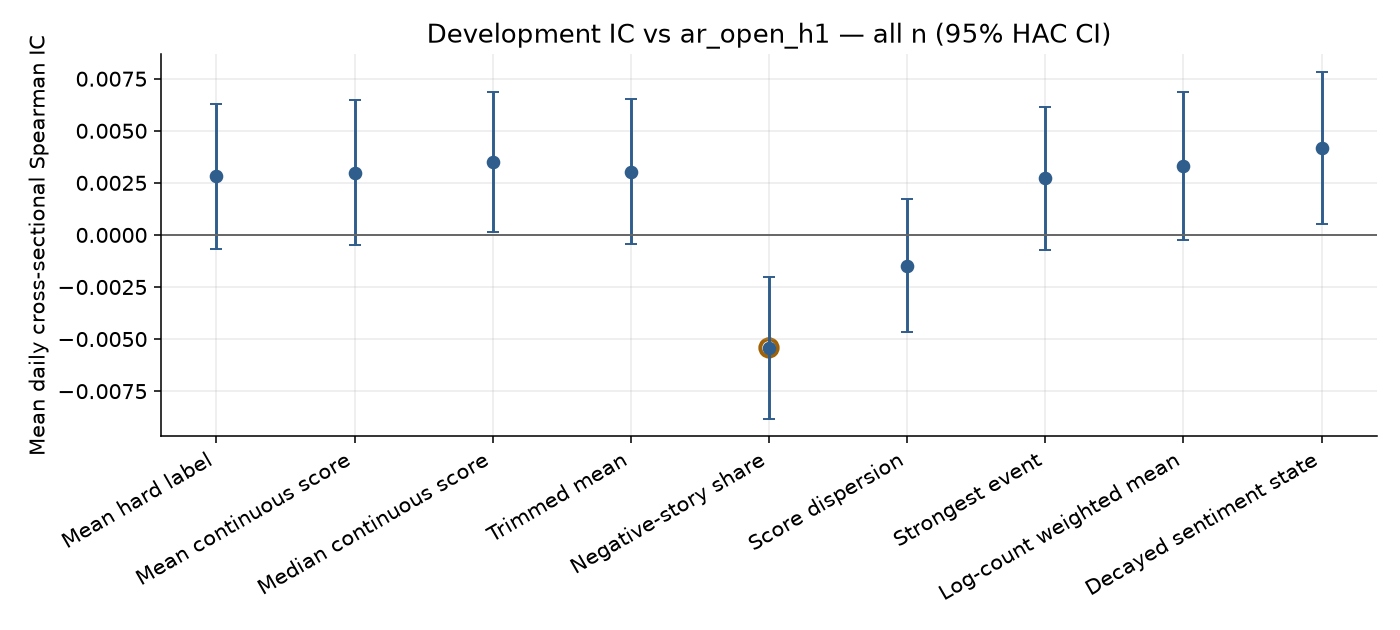
\includegraphics[width=\textwidth]{fig_aggregation_ic}
  \caption{Mean daily cross-sectional rank correlation between each aggregation rule and the next-open abnormal return, development period, with 95\% HAC intervals. Negative-story share is the only rule that survives the multiplicity correction.}
  \label{fig:aggregation-ic}
\end{figure}

\section{Information Beyond the Mean}
\label{sec:results-conditional}

\draftnote{Report Notebook 71 as the direct primary estimand, not as another aggregator tournament. Across 2{,}264 FNSPID development sessions and 512{,}149 complete firm-days, the mean daily coefficient on negative-story-share rank is $-0.008310$ after controlling for mean continuous sentiment rank and log news-count rank. The HAC(5) 95\% interval is $[-0.014100,-0.002520]$ and $p=0.004907$. This is the clean evidence for ``beyond the mean''. Keep the interpretation in rank units and avoid implying a causal return effect.}

\section{Costs and Learned Thresholds}
\label{sec:results-costs}

\draftnote{Daily trading turns the book over roughly 200 times a year and the best break-even across the nine rules is 0.625 bps per side against the 10 bps charged; every net Sharpe is negative. Learned thresholds (logistic, gradient-boosted, MLP) sit at evaluation AUC around 0.50 and cash beats every learned policy, which closes the secondary question. Source: Notebooks 03, 10.}

\begin{figure}[htbp]
  \centering
  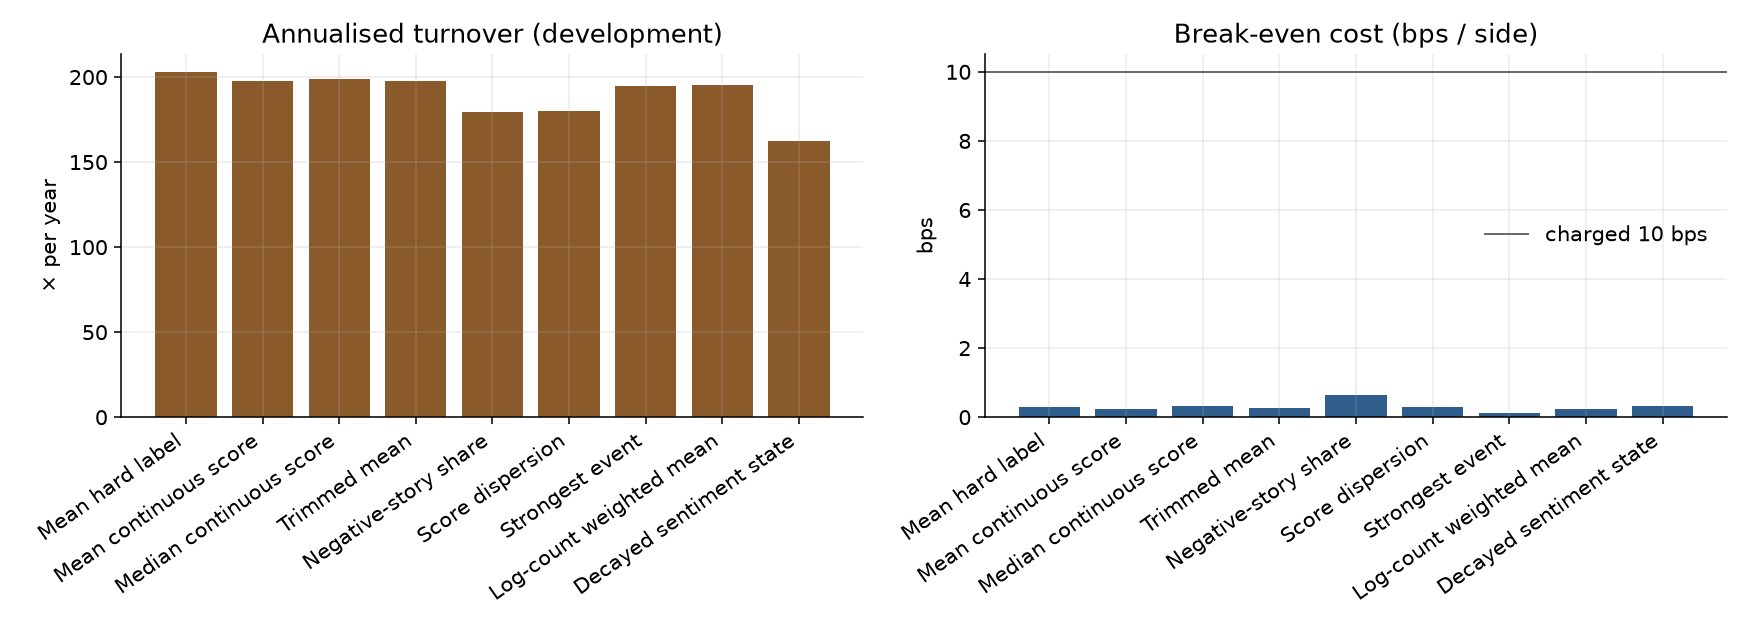
\includegraphics[width=\textwidth]{fig_turnover_breakeven}
  \caption{Annualised turnover and break-even transaction cost for each aggregation rule on the development block. The best break-even is 0.625 bps per side; the charged cost is 10 bps.}
  \label{fig:turnover-breakeven}
\end{figure}

\section{The Signal as a Risk State}
\label{sec:results-risk}

\draftnote{HAR base: evaluation net Sharpe 0.673, maximum drawdown $-15.73\%$, against 0.568 and $-32.05\%$ for buy-and-hold SPY. The hysteresis overlay lifts net Sharpe to 0.835 and total return from $+29.85\%$ to $+35.20\%$ at 2 bps per side, stays ahead at 10 bps, and reduces downside-squared loss ($p=0.0148$); the paired return interval spans zero. Walk-forward 2013--2019: drawdown $-12.53\%$ to $-8.57\%$ ($p=0.0052$), mean return slightly worse. The exact LSEG transfer in Notebook 72 never crosses the frozen 1.5 entry threshold (maximum z-score 1.349; 0/167 risk-off sessions), so overlay and HAR are identical at net Sharpe 0.240. Sentiment times risk is a one-regime result, not a portable rule.}

\begin{figure}[htbp]
  \centering
  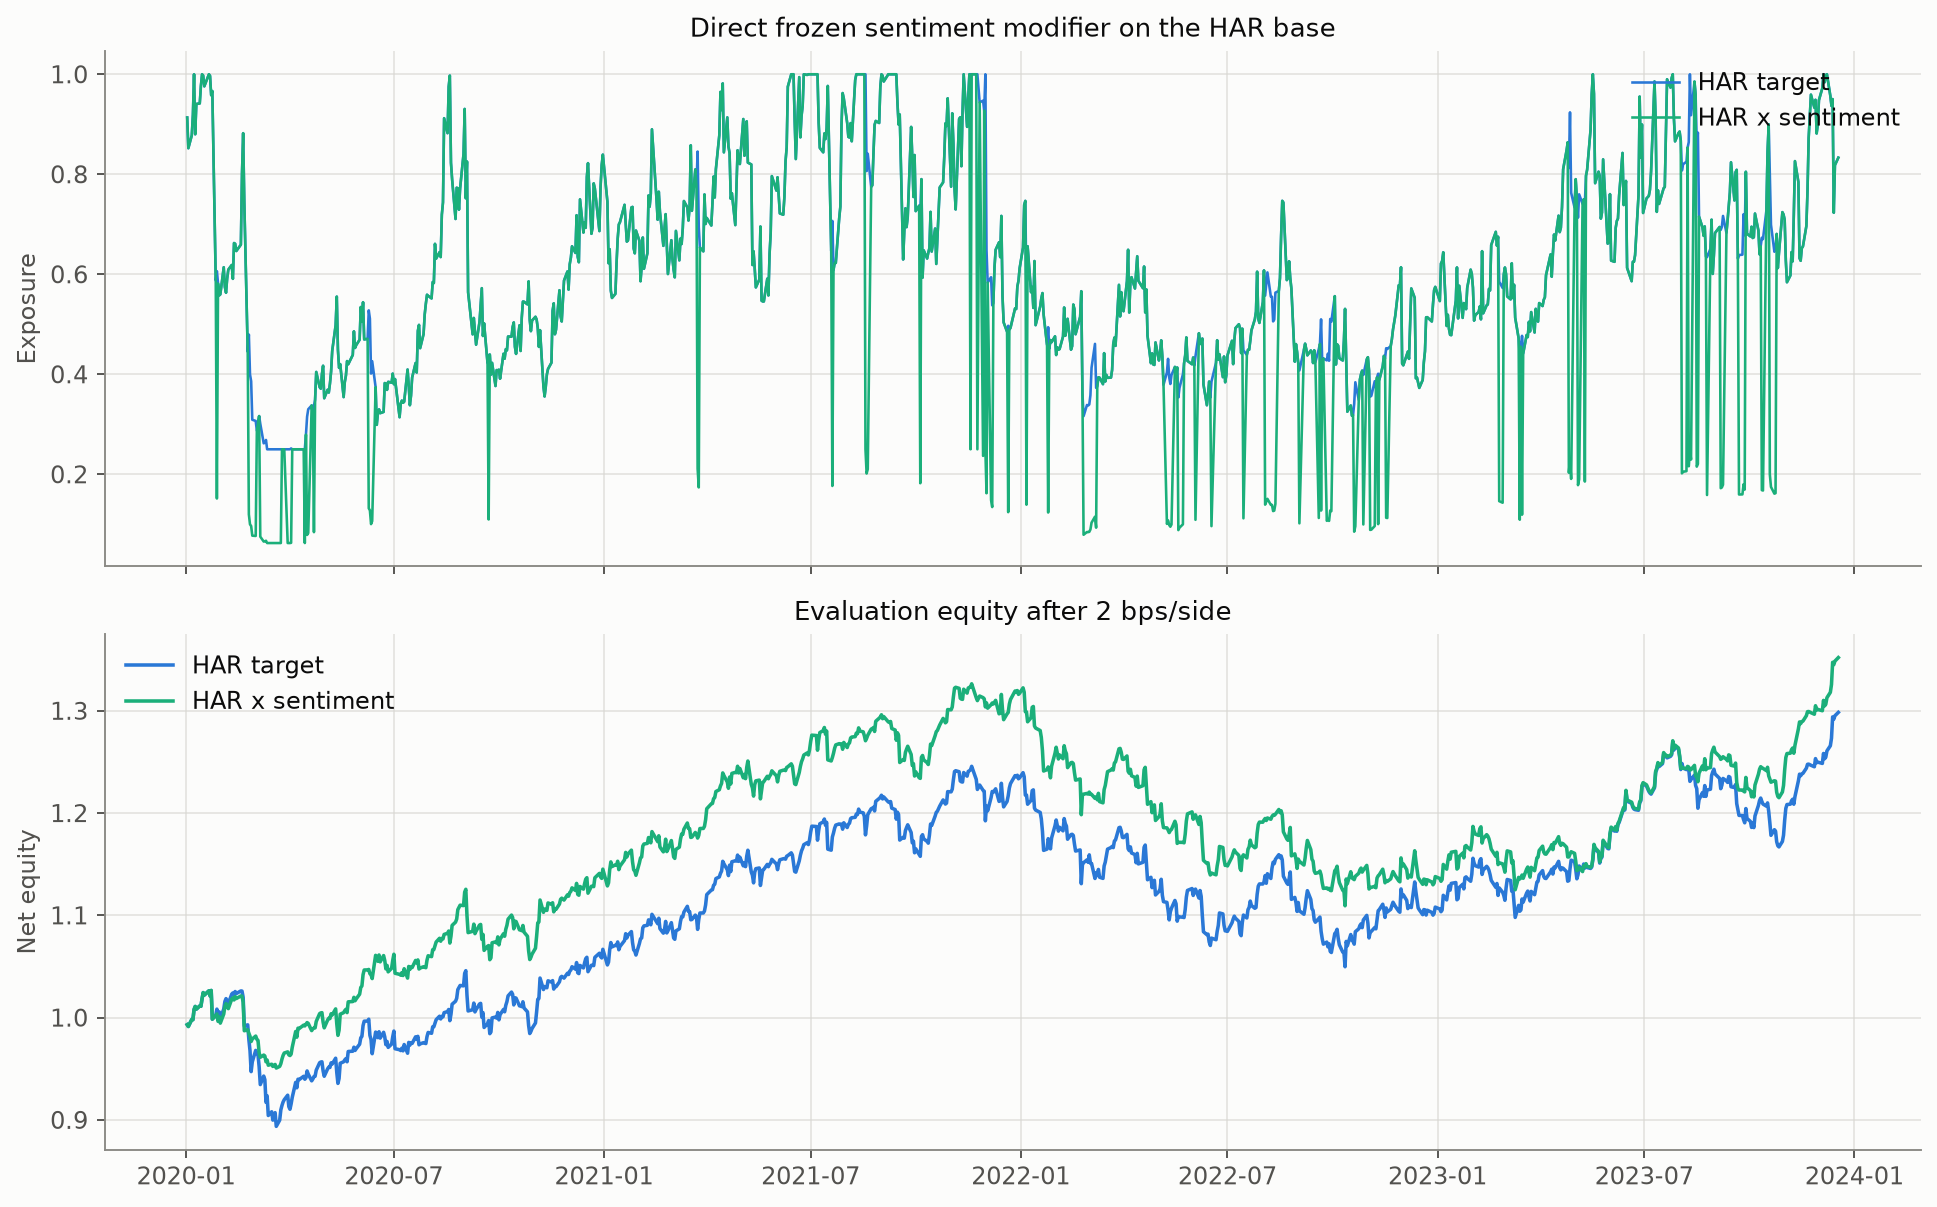
\includegraphics[width=\textwidth]{fig_har_sentiment_equity}
  \caption{The HAR volatility target and the same target scaled down when aggregate negative-story pressure is high, evaluation period 2020--2023, at 2 bps per side.}
  \label{fig:har-sentiment}
\end{figure}

\section{Placebo Boundary}
\label{sec:results-placebo}

\draftnote{Circular-shift placebo: the observed schedule beats 99.1\% of placements in 2020--2023 (exact $p=0.0100$, BH $q=0.0301$), is suggestive but uncorrected in 2013--2019 ($p=0.0455$, $q=0.0682$), and is ordinary in the LSEG 2025--2026 window. The claim is one-period downside timing, stated with exactly that boundary. Source: Notebook 45.}

\begin{figure}[htbp]
  \centering
  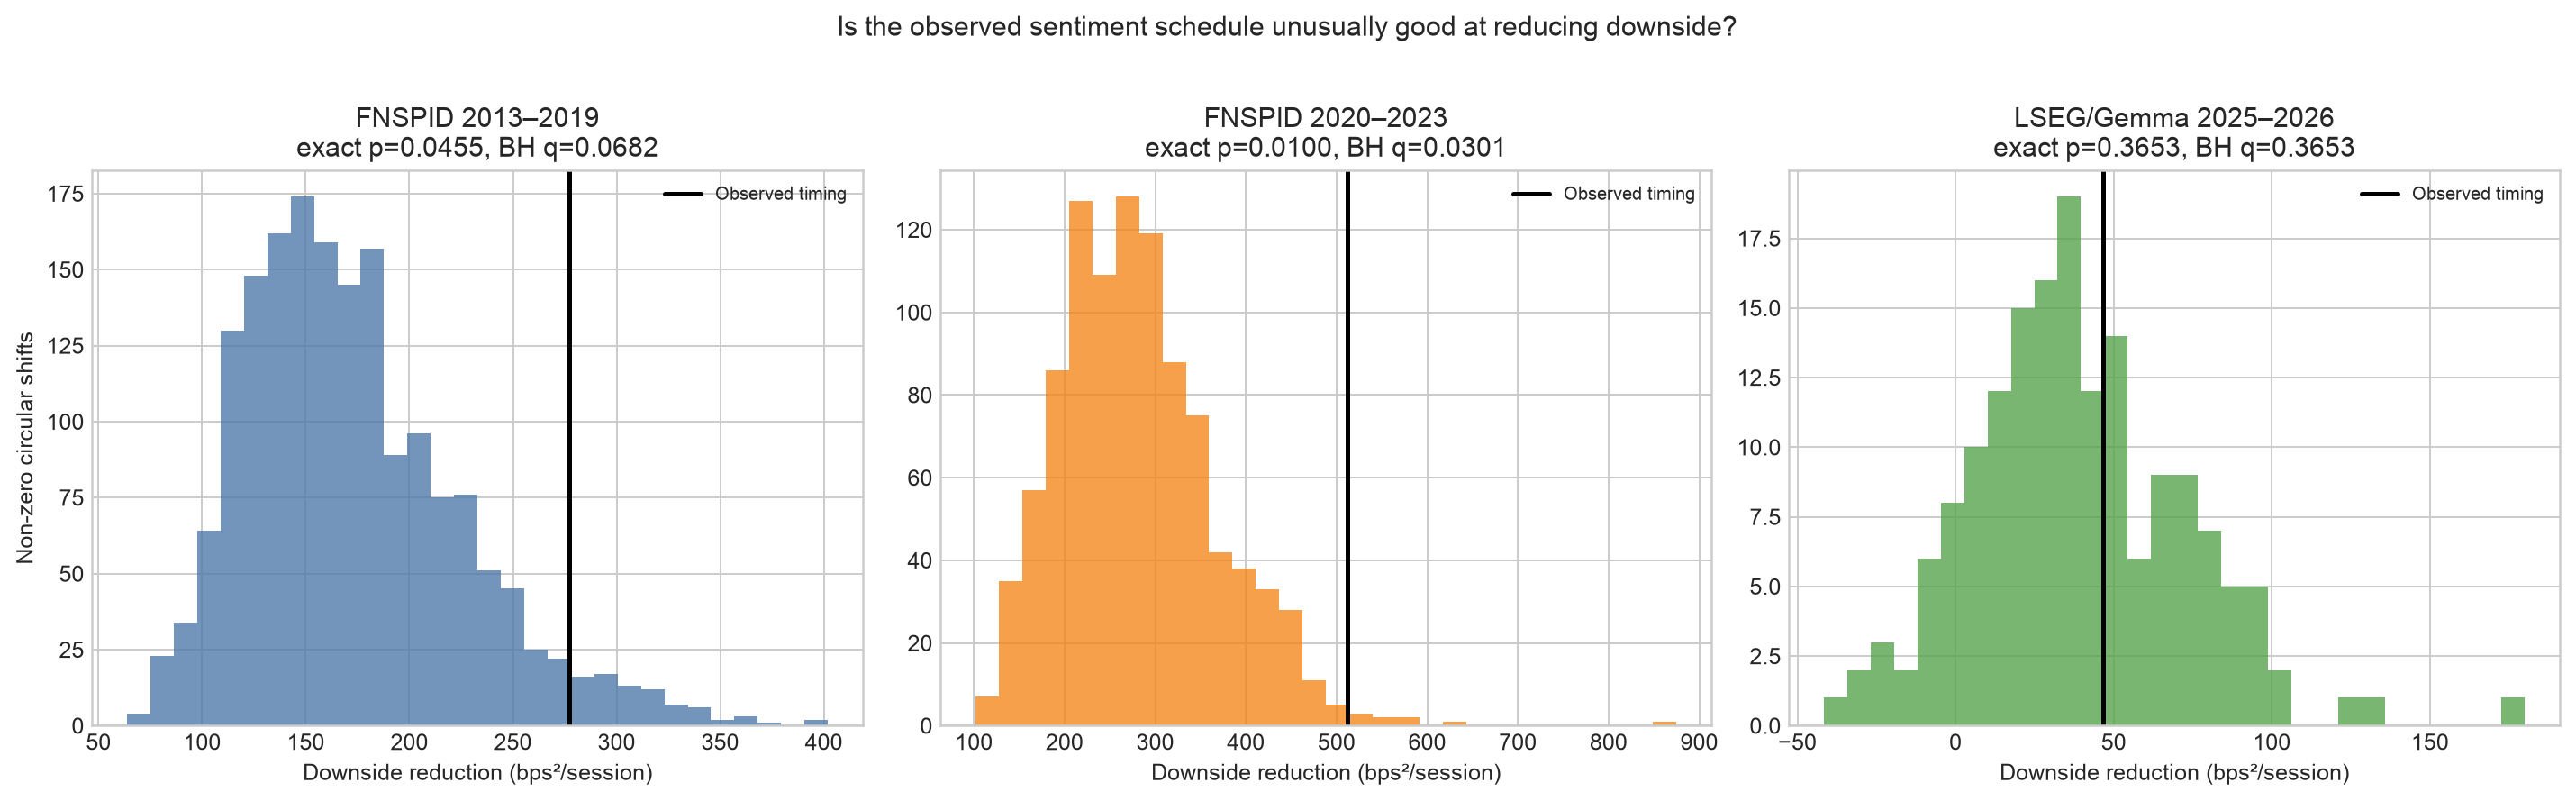
\includegraphics[width=\textwidth]{fig_downside_placebo}
  \caption{Downside reduction of the observed sentiment schedule (vertical line) against every non-zero circular shift of the same schedule, in three separate regimes. Only 2020--2023 survives the correction.}
  \label{fig:downside-placebo}
\end{figure}

\section{Robustness from a Second Source}
\label{sec:results-robustness}

\draftnote{One compact section on the non-pooled LSEG regimes: the five-arm sector-33 and midcap-22 nulls, and the temporal-fragility result. The hybrid selected on the opened 2025--2026 window earned net Sharpe 2.271 there and $-0.354$ on an earlier block of the same 33 names; the portable continuous rule was net-negative in both blocks while headline-level scores stayed highly rank-repeatable (Spearman 0.989). Then report the more relevant RQ-A transfer: pinned-FinBERT negative-share conditional coefficients are negative in both LSEG blocks ($-0.02861$ backward; $-0.01573$ recent), but 95\% intervals $[-0.07283,+0.01560]$ and $[-0.09453,+0.06308]$ cross zero after the two-block family. Their 10-bps books lose. Stable or directionally similar measurement does not by itself produce precise portability or a cost-covering signal. Sources: Notebooks 11, 13, 36, 67, 70--72.}

\chapter{Conclusions and Future Directions}
\label{ch:conclusion}

\section{Answers to the Research Questions}
\label{sec:conclusion-answers}

\draftnote{Answer the primary and secondary questions directly with the main estimates and their uncertainty, then state the composite conclusion: in FNSPID development, the distribution beyond the mean carries detectable negative-tail information even after mean sentiment and news count are controlled; the result is not economically usable as a directional signal at realistic costs; the downside-risk evidence is bounded to one FNSPID period; and neither the conditional coefficient nor the exact risk-state rule is established as portable to LSEG.}

\section{Strengths, Weaknesses and Future Work}
\label{sec:conclusion-future}

\draftnote{Strengths: one inference regime, declared multiplicity, explicit costs, placebo boundary, nulls as results. Weaknesses: exploratory-not-confirmatory history, chronological-not-pristine split, machine labels without human validation. Future directions: the registered prospective LSEG replay (earliest completion December 2026) and the sealed materiality confirmation as specified confirmatory tests.}

\addcontentsline{toc}{chapter}{Bibliography}
\bibliographystyle{ormsv080}
\bibliography{references}

\appendix

\chapter{Reproducibility Record}
\label{app:reproducibility}

\draftnote{Populate from the frozen manifests in \texttt{final\_experiments/outputs/}: Git commit, input and configuration hashes, model identity, split definition and output hashes for each result promoted into \cref{ch:results}. Include the programme-required artificial-intelligence use statement. Do not paste proprietary FNSPID or LSEG text.}

% REQUIRED BEFORE SUBMISSION: insert the final project summary here, after the
% appendices, using the programme's current 2026 wording and format.

\end{document}
